% !TEX root = dissertation2.tex
\chapter{Methodology}
%Purpose of Study
The researcher sought to determine the viability of RTK GNSS augmentation to asses railway infrastructure and act as a reliable track vehicle locator capable of meeting the requirements of a location determination system as defined by the FRA by answering these questions:

1)\emph{Hump Yard Profile:}
Can a locomotive use RTK augmented GPS to measure the  vertical profile of bowl tracks in an automatic classification yard during production activities?

2)\emph{Horizontal Track Alinement:}
Can a common track vehicle use RTK augmented GPS/GNSS to determine the horizontal degree of curvature ($D_c$) comparable with specialized track geometry vehicles?

3)\emph{Track Occupancy:}
Can a common track vehicle use RTK augmented GPS/GNSS to meet the positioning requirements for track occupancy outlined by the FRA~\citep[pp.6-7]{1995FRADiffe} for a location determination system?

The researcher evaluated the capability of Real Time Kinematic (RTK) augmentation applied to Global Navigation Satellite Systems (GNSS) to safely, rapidly, and precisely measure track position employing common track vehicles such as Hi-Rails and locomotives as a survey platforms. Figure~\ref{fig:plan} describes the major goals and their relationship in meeting the research objectives. Rail transportation needs were identified from interviews with rail company experts; an assessment of current railroad process and capabilities; observation of yard operations in light of the expert interviews; and the identification of a statewide CORS network accessible to researchers. Interviews with subject matter experts has led to the design of experiments that were performed within the safety and access constraints of a Class I railroad.

This chapter contains the method for how:
\begin{enumerate}[1)]
	\item A hump yard was profiled by an RTK GPS equipped locomotive to measure track position during humping operations.
	\item A RTK GNSS equipped Hi-Rail was used to define ${D_c}$ across 29 continuous miles of mainline track.
	\item Multiple traverses by a RTK GNSS equipped Hi-Rail were evaluated for the statistical likelihood of reliably determining track occupancy in parallel multitrack segments.
	
\end{enumerate}

% Research Design
\section{Research Design and Data Collection}
The research investigated the use of RTK augmentation to the GPS and to GPS plus GLONASS (Referred to collectively as GNSS).
% Research Plan Diagram
\begin{figure}[!h]
	\centering
	\includegraphics[width=6in]{graphics/research_plan.png}
	\caption{Research Plan}
	\label{fig:plan}
\end{figure}
The research investigated the capabilities of RTK GPS/GNSS over active track. Due to federal and private property laws restricting access to active track, all research activities were performed adhering to the provisions of 49 CFR \S214 railroad workplace safety regulations, subpart C \textit{Roadway Worker Protection}~\citep{49CFR214300} and subpart D \textit{On Track Roadway Maintenance Machines and Hi-Rail Vehicles}~\citep{49CFR214500} as well as specific rail company rules and procedures set out by the employee in charge during job safety briefings. 

Track location of bowl tracks in a hump yard was determined from single epoch track observations from a GPS mounted on a locomotive traversing an active hump yard. The track positions were used to produce profiles for each bowl track in the yard. Relative vertical precision and base station observations were used to evaluate the yard environment for RTK GPS surveying by locomotive.

An evaluation of RTK augmented horizontal performance was made by single epoch observations of track position by RTK GNSS receivers mounted to a track inspector's Hi-Rail traversing active mainline track. Horizontal track alinement was evaluated by means of a software modeling the string lining method to determine the degree of curve from single epoch RTK GNSS track position observations. Degree of curve ($D_c$) determined by the RTK GNSS string line model was compared with $D_c$ determined by a track geometry car over an identical tangent segment.

An evaluation of RTK GNSS to determine track occupancy was made by multiple Hi-Rail traverses with RTK GNSS instruments across multiple parallel segments of mainline track. Positions observed over identical and parallel segments of tangent and circular track were evaluated for cross-track error\footnote{per Allen et al., \pageref{fig:trackRef}} for the likelihood of determining track occupancy by an RTK GNSS equipped mobile rail vehicle.

The electrical point of reference for a GPS/GNSS antenna is the phase center. The phase center is offset some distance from a physical reference location on the antenna housing. The physical antenna reference for each of these experiments was the mounting surface or antenna reference point (ARP). The survey controller contains a table of offset distances between phase center and ARP for the antennas used during each experiment. A procedure to align the ARP on the track vehicle to a selected railway reference location\footnote{i.e., Track centerline, left (port) gauge side or right (starboard) rail.} was performed as part of the mobile track vehicle setup.

Estimates for the relative horizontal and vertical precision\footnote{Relative errors are errors and precisions expressed for and between pairs of network adjusted control points.} are calculated by the \emph{Survey Controller} software in the Trimble TSC2 controller. \emph{Trimble Survey Controller} software uses a algorithm to compute vertical precision:
	\begin{equation}
Vertical Precision (m) = ErrorScale * VDOP * ScaleFactor\\
	\end{equation}
Where:\\
${ErrorScale = \frac{\sqrt{ErrorE + ErrorN + ErrorU}}{PDOP}}$\\
ErrorE = CovENU[x][x]\\
ErrorN = CovENU[y][y]\\
ErrorU = CovENU[z][z]\\

Where CovENU is the aposteriori covariance matrix of the RTK solution from the RTK engine in the GNSS receiver.\\
\emph{ScaleFactor} is either 1 or 1/3 depending on whether the RTK engine is giving \emph{Survey Controller} 1-sigma or 3-sigma precisions, which depends on the version of RTK engine. The \emph{Survey Controller} display shows 1-sigma precisions.\\

The observation procedure for these experiments progress from setup of an ad hoc  reference station in the case of experiment 1, or accessing a VRS reference network as in experiments 2 and 3; establishing a means of communication between the reference station/VRS and the track vehicle; aligning the antenna with a track reference point; and configuring the mobile receiver onboard the track vehicle.

%Hump yard profile design
\subsection{Experiment One: Hump Yard Profile Survey} \label{ResDHmpYd}

Experiment one asked whether RTK augmented GPS mounted to a locomotive could measure the  vertical profile of bowl tracks in an automatic classification yard without the need for track closures.

The objective of experiment one was to use RTK GPS instrumentation mounted to a locomotive to survey an active hump yard in order to produce track profiles. The survey data was used to create information products which were handed off to the rail company sponsor in preparation for a yard-wide resurfacing project.
%{Ad Hoc Base Station Procedure}

Coordinates are reported as in US survey feet,
\begin{description}
	\item System: US State Plane 1983.
	\item Zone: North Carolina 3200
	\item Datum: North American Datum 1983
	\item Geoid: Continental United States 2003
\end{description}

The hump yard survey used a single RTK reference station transmitting correctors via UHF radio to a mobile receiver onboard a locomotive.  The ad hoc reference station components are listed in table \ref{tab:instruments}. A fixed-height tripod at 1.5 meters supported the GPS and UHF antennas. The ad hoc reference station was set on top of a two story masonry structure to maximize height above average terrain (HAAT) for UHF data reception by the roving receiver aboard the locomotive as shown in figure figure \ref{fig:AhRS}. The elevated location provided sufficient HAAT to enable reception of correctors across the yard and to NGS benchmark EB1559 located 8,500 feet from the 25 watt UHF transmitter.

The autonomous horizontal position of the reference station (CP1) was adjusted by using the results of NGS OPUS from observations recorded during two sessions. The first session was 2008/05/26 14:21:00 to 21:44:00 UTC with the second session 2008/05/27 12:12:00 to 18:50:00 UTC\label{baseRefPeriod}. The compressed observation files were converted\footnote{Using Trimble \emph{runpkr00} under Unix.} to the Receiver INdependent EXchange (RINEX) format and submitted to the National Geodetic Survey Online Position User Service (NGS OPUS) for position determination. The autonomous horizontal position of the ad hoc reference station (CP1) was adjusted to the mean northing and easting of the two NGS OPUS reports exhibited in Appendix A, pages \pageref{opus1}-\pageref{opus2}.

The autonomous vertical position of the reference station was adjusted using RTK observations on a NGS benchmark, permanent identifier (PID) EB1559. The benchmark was located 8,508 from the ad hoc RTK reference station. The elevation of CP1 was adjusted to minimize the difference between the observed and the published NAVD88 elevation for the first order class II\footnote{\citep{FGCCstds}} benchmark. The PID datasheet for EB1559 is exhibited in Appendix A, pages \pageref{EB1559-1}~-~\pageref{EB1559-3}.

Multipath concerns were examined at the reference stations by generating a full TEQC~\citep{TEQCsoftware} (Translation, Editing, and Quality Check) report from the reference station RINEX observation and navigation files. The TEQC reports are exhibited in Appendix A.

% AhRS setup photo
\begin{figure}[!h]
  \begin{center}
    \includegraphics[scale=0.5]{graphics/AhRS_hamlet_BW}
   \caption{Ad hoc Reference Station}
  \label{fig:AhRS}
\end{center}
\end{figure}

An EMD SD60 yard locomotive was equipped with the mobile\#1 instrument indicated in table \ref{tab:instruments}. The mobile GPS antenna mount was collocated with an omnidirectional UHF antenna and secured to a SECO magnetic base as illustrated in figure \ref{fig:locoAnt}. The antenna mount was fitted with a wire rope safety lead to secure the antenna assembly to a fixed member on the locomotive cab to prevented injury to locomotive operators or ground personnel in the event the antenna was dislodged by handling rail cars. The antenna were  connected to the mobile receiver with ten-foot lengths of RG-58 50\ohm~coaxial cable.

% AhRS setup photo
\begin{figure}[h!]
  \begin{center}
    \includegraphics[width=0.48\textwidth]{graphics/AntennaMountBWcrop}
  \end{center}
  \caption{GPS/UHF Antenna Setup on Locomotive}
  \label{fig:locoAnt}
\vspace{-20pt}

\end{figure}
The antenna was aligned with the track centerline in an area designated by the yardmaster and blue flagged during installation to insure the safety of research and railroad company personnel working around the locomotive. The generalized procedure for aligning a GPS/GNSS antenna mounted to a track vehicle with a horizontal track reference and determining the antenna reference point from the top-of-rail elevation is described following and referencing figure~\ref{fig:antAlign}.

% Antenna alignment procedure
\subsubsection{Antenna Alignment Procedure}
\label{Antenna Alignment}
\begin{enumerate}
\item A job safety briefing is conducted by the rail company employee-in-charge.
\item A frequency in the 450~Mhz band is selected by monitoring voice traffic on available channels, as data is a secondary use of this spectrum. The ad hoc reference station is programed with an autonomous position, and corrector transmission initiated.
\item  A section of tangent track approximately 300 feet long is blue flagged and made safe by setting a derail and locking out the track switch as discussed during the job safety briefing.
\item Track centerline points are measured on either end of the calibration area, figure~\ref{fig:antAlign} points A and A'. The centerline points are observed with a Trimble R8 instrument for 180 epochs.
\item A line feature representing the track centerline is created in the survey controller between points A and A'.
\item The center point of the line feature is determined. Two points, referenced in figure~\ref{fig:antAlign} as points B and B', are observed at the the top of each rail for 180 epochs.
\item A second line feature between points B and B' is created in the survey controller.
\item A point located by intersecting lines A-A' and B-B', figure~\ref{fig:antAlign} point C, is determined by the \emph{Survey Controller} software.
\item The mean elevation of the top of rail observations is calculated and assigned to point C.
\item The GPS/UHF antennas and magnetic base mount are placed in the approximate center of the top of the locomotive cab. A wire rope safety harness connecting the antenna mount to the locomotive horn or other suitable anchor point is secured.
\item The survey controller is connected to the GPS receiver in the track vehicle. The previously created data file with the alignment features described above is opened.
\item Blue flags are removed from the locomotive by the persons that placed them. Derails are stowed and facing point track switch operators are unlocked. Movement authority is obtained from the yardmaster by the locomotive engineer.
\item The locomotive is moved to locate the GPS/UHF antenna mount over point C.
\item The locomotive is secured and the antenna mount moved in small increments to intersect the centerline by observing the instantaneous antenna location in the map view of the controller. A period of  ten seconds between movements is allowed for the position to settle in the map display.
\item The survey controller antenna height is set to zero. Figure~\ref{fig:antAlign} point D is observed for 180-epochs. An inverse calculation is performed between points C and D. The elevation difference is recorded as the antenna height.
\item A survey style is created in the \emph{Survey Controller} software containing the antenna height above the top-of-rail elevation. Due to variation in cab height above top-of-rail, the survey style is named for the particular locomotive unit number used in the antenna alignment. Likewise for individual Hi-Rail vehicles.
\end{enumerate}

% Alinement drawing
\begin{figure}[h!]
  \begin{center}
    \includegraphics[scale=0.40]{graphics/antennaAlinement.png}
  \end{center}
  \caption{Track Vehicle Antenna Alinement Procedure}
  \label{fig:antAlign}
\vspace{-20pt}
\end{figure}

RTK correctors were broadcast from the single reference station by UHF data radio and used to augment the GPS receiver aboard the locomotive. A survey controller connected to the receiver managed and automated data collection by recording single epoch observations with a nominal horizontal separation of ten feet. Track profiles originated at a common reference point at the hump end of the bowl and terminated at the pullout-end switch for each track.

The pullout end of the bowl was surveyed first, from pullout switch to foul point\footnote{The track foul point is the demarcation between hump and pullout end movement authority.}. The hump end of the bowl was surveyed during a shift change, from the hump to foul point, to minimize disruption to humping operations. Locomotive movement across the pullout end of the yard was coordinated between the locomotive operator and pullout end humpmaster\footnote{Responsible for outgoing train makeup and movement.}. Track traverses began at the pullout end switch and progressed to the foul point. The automatic numeric sequencing of the survey controller was used to produce unique point identifiers. The controller sequence was constructed by concatenating: 1) the  two digit track number; 2) a single digit traverse counter; 3) a three digit point sequence beginning at 000 and incremented by one at each observation in sequence. Points recorded onboard the locomotive were feature coded as centerlines.

The hump end survey was performed in coordination with the hump end humpmaster\footnote{Responsible for railcar sequencing and switching into the bowl.} during the yard shift change to minimize the impact of the survey interrupting yard production. The locomotive traverse of the hump end began at the hump, through the retarder and track leads, finishing at the track foul point. The unique point identification scheme previously described was not performed due to time constraints. The hump, leads, and track points were separated post survey.

Points of interest (POI) were surveyed on the ground with the static module referenced in table \ref{tab:instruments}. The static receiver was mounted to a 2 meter range pole. Multiple epoch observations (3-6) were recorded at each point of interest. Feature codes distinguished switch points, wheel detectors, retarder inlet/outlet, and foul points. Switch points and retarders were identified by rail company reference number. Wheel detectors were identified by track and sequence number. Ground point safety was superintended by a rail company employee.

% Hump Yard Data
\emph{Variables of analysis}: The mobile instrument \#1, table \ref{tab:inst} produced these variables:
\begin{itemize*}
\firmlist	
	\item US State Plane, North Carolina 3200, northing in US survey feet.
	\item US State Plane, North Carolina 3200, easting in US survey feet.
	\item NAVD 88, height above ellipsoid 2003, in US survey feet.
	\item Vertical precision estimate determined by \emph{Survey Controller} software, in US survey feet.
	\item Time (local, EST) and date of observation.
	\item A count of the SVs in view of the mobile\#1 GPS antenna.
	\item Vertical Dilution of Precision (VDOP)\footnote{A unitless figure of merit expressing the relationship between error in in user position, and the error in satellite position. PDOP is related to the horizontal and vertical PDOP by: ${PDOP = \sqrt{HDOP^2 + VDOP^2.}}$} determined by \emph{Survey Controller software}
\end{itemize*}

Yard observations were exported from the \emph{Survey Controller} software and separated into layers organized by lead, group, and track. Deconstructing the aggregate observations enabled individual tracks to be configured as a continuous series of points by activating the particular layers in TGO.
\begin{itemize}
\item Hump lead
\item Main retarder
\item Intermediate retarders
\item Group retarders
\item Group leads
\item Bowl tracks
\end{itemize}
A properly configured track was apparent as a continuous series of points extending from the hump through the desired track to the pullout end switch.

Locations of track POI (i.e., track switch points, retarder inlet and outlet, wheel detectors) were associated with a position nearest a particular rail. The POI was observed at the center top-of-rail nearest the POI physical location using the static survey instrument. The position of each POI was adjusted post survey to be coincident with the track centerline.

Continuous track observation names were renumbered in the TGO software, in series progressing from hump to pull out. Feature codes enabled separation by feature. The \emph{TGO} software was used to create line work by connecting consecutive centerline points. The line work and observation data were exported from TGO in the ESRI\footnote{Environmental Systems Research Institute, Inc.} shapefile format. The point data was also exported as a comma delimited (CSV) format and imported to a \emph{Google Docs} spreadsheet. A linear reference was determined for each point according to equation \ref{eq:horzSta}. Elevations and linear references were scaled and input as an overlay to a CAD drawing containing the track design grade\footnote{Provided by the rail company sponsor.}. 

Each track profile was plotted as an overlay to the provided CAD drawing. The design profile in the CAD drawing is relevant to the rail company in a making a volumetric assessment of surfacing material required to bring the relief of each track into vertical alignment with the design grade. Calculation of surfacing material quantity is outside the scope of the experiment. The design grade and locomotive survey result will be used as a comparative tool, limited to providing track profile deviation from design grade.

The shapefiles will be added to ESRI ArcMap software where a plan view of of the bowl area track elevation and vertical precision estimate will be represented in plan view. The vertical precision map will show lower quality vertical precision for points > 0.1 feet in a contrasting color to those of greater precision. The plot will be examined for the distribution of lower quality data patterns.

Acceptable elevation quality will be apparent as a smooth track profile. Poor quality observations will appear with greater variation between points, resulting in a jagged or sawtooth profile. Poor quality elevations will be identified and correlated with: observation time; vertical precision estimated by the receiver; and reference station observations during the period.

The vertical precision calculated by the \emph{Survey Controller} software was used to determine descriptive statistics and to plot a histogram for analysing the quality of GPS observations by the mobile instruments.

%Horizontal stationing equation
	\begin{equation}
	{sta_k} = {match~point~offset} + {\sum_{k=2}^n}  {\sqrt{(x_k - x_{k-1})^2 +( y_k - y_{k-1})^2}}
	\label{eq:horzSta}
	\end{equation}
\begin{quotation}
Where \emph{k} =  a point in the ordered sequence of observations, and \emph{n} = the number of observations in the track segment, and the match point offset is the horizontal distance from the top of the hump to switch point 1574.
\end{quotation}

Experiment one:
\begin{enumerate}
	\item Produced an alignment procedure for alignment of the GPS antenna with the centerline top-of-rail location.
	\item  Collected continuous single epoch observations on a nominal 10 foot horizontal spacing with RTK augmented GPS onboard a locomotive in an active hump yard. 
	\item Resulted in the production of a plan-view color-map of track elevation for the bowl area of a hump yard.
	\item Resulted in the production of a plan-view color-map of relative vertical precision as determined by the \emph{Survey Controller} software for points measured in the bowl area of the yard.
	\item Resulted in the production of a two-dimensional profile drawings for each track in 1:1 and 1:5 vertical scale.
	\item Determined the descriptive statistics of the relative vertical precision as determined by the \emph{Survey Controller} software for the locomotive mounted GPS .
	\item Resulted in the production of TEQC reports for two ad hoc reference station observation sessions.
\end{enumerate}

% Mainline Track alinement design
\subsection{Experiment Two: Determining Horizontal Track Alinement}
\label{Ex2Design}
This research asks whether RTK augmented GPS and GNSS instruments mounted to a common track vehicle can determine horizontal track alinement comparable those acheived by specialized track geometry vehicles. The objective of the experiment was to perform multiple mainline track surveys with RTK instruments mounted to a Hi-Rail vehicle; the development and demonstration of a software model using the string lining procedure in order to produce horizontal track alinement. The track alinement survey employed a series of CORS RTK reference stations along the survey route, networked to the Ohio Department of Transportation, Aerial Mapping Virtual Reference Station (ODOT VRS) server.

The ODOT VRS was used to minimize the $\pm$1 ppm error incurred as distance increases from a reference station. The VRS creates a new virtual reference station when the baseline between the track vehicle and the previous VRS created reference station increased beyond a distance programmed in the VRS. A public cellular data service was used to exchange security credentials with  the ODOT VRS server, receive correctors, and apply them to a mobile receiver onboard a track inspector's Hi-Rail. A survey controller connected to the mobile receiver recorded single epoch observations with a nominal horizontal point separation of five feet with mobile instrument\#2 (table \ref{tab:instruments}) and ten feet with mobile instrument\#1. Nominal point separation was based on the receiver processing speed for Hi-Rail traverses in the range of 10 to 30 mph.

% Alinement Study Area
Two mainline track segments of different character were traversed during this experiment. The first segment can be characterized as multiple parallel track, signalized, Class 4, with a maximum allowable track speed between 30 and 50 mph, carrying a freight volume of 25 to 35 MGT/yr\footnote{Million Gross Tons per year}. This segment is referenced as C\&O Kanawha subdivision, from mile post 494 to 523 (MP494-523). Continuous observations over this segment demonstrates the capability of an RTK VRS over a wide area.

A second segment, characterized as single track, dark territory, Class 3, with allowable track speed between 10-30 mph, carrying a freight volume of less than 10 MGT/yr, is referenced as C\&O Ohio River subdivision from mile post 210 to 207 (MP210-207). This segment was selected for study as the segment had been examined previously by Szwilski~\citep{Szwilski03}. Additionally, data was made available from CSX's Gauge Restraint Measurement System\footnote{A specialized, self-propelled, track geometry car.} (GMRS) across this segment. Degree of curvature (${D_c}$) from the GMRS was compared with the horizontal alinement model by selecting a tangent segment for comparision. An ideal measurement across a tangent segment would result in a ${D_c}$ of zero. Therefore, the ${D_c}$ deviation from zero across the tangent segment was used to compare the GMRS measurement with RTK modeled ${D_c}$ measurements.

% FRA alinement figure
\begin{figure}[!htp]
	\vspace{-30pt}
		\begin{center}
			\includegraphics[width=3in]{graphics/HorzAlignment.png}
			\caption{Horizontal Alinement}\label{fig:Alinement}
		\end{center}
	\vspace{-30pt}
\end{figure}

The track observations were used as inputs to a software to determine the ${D_c}$ modeling the FRA guidance manual instructions for using the string line method.
Experiment two objectives sought to:
\begin{enumerate}
	\item Collect continuous single epoch observations with RTK augmented GPS/GNSS mounted to a track inspector's Hi-Rail over at least 29 continuous miles of mainline track. Point spacing was a nominal 10 foot for mobile configuration\#1 and 5 foot horizontal spacing for mobile configuration \#2 (see table \ref{instruments}).
	\item Develop a software model for calculating degree of curvature (${D_c}$) from RTK augmented GPS/GNSS track vehicle observations. The software model replicated the string lining method described in FRA \emph{Track Safety Standards Compliance Manual}~\citep[pp.26-30]{2007FRATrack} using a 62 foot chord length and 15.5 foot stations.
	\item Compare two methods of measuring ${D_c}$ over tangent track. The first method utilized data from a specialized track geometry car, CSX's GMRS. The self propelled GMRS was designed specifically for the purpose of obtaining ${D_c}$ (and other track alinement parameters\footnote{Gage, crosslevel, profile, ${D_c}$}) from the string lining method. The second method utilized data obtained from an RTK GNSS instrument mounted to a track inspector's Hi-Rail and a software to model the string line method from the Hi-Rail data.
	A traverse of identical tangent track segments was compared for cross-track\footnote{See Allen, et al., figure \ref{fig:trackRef}, page \pageref{fig:trackRef}} centerline deviation using descriptive statistics. Identical segments were determined by selecting beginning and ending mile post reference locations.
	\item The ${D_c}$ was determined and track elevation measured using RTK survey equipment mounted to a track inspector's Hi-Rail across a continuous 29 mile track segment. The modeled ${D_c}$ was compared with company supplied track charts to correlate the location and magnitude of curves. Structures responsible for loss of signal (LOS) were identified.
\end{enumerate}

\emph{Variables of analysis}: The mobile instrument \#1 and \#2, table \ref{tab:inst} produced these variables:
\begin{itemize*}
	\item UTM, Zone 17 North, northing in US survey feet.
	\item UTM, Zone 17 North, easting in US survey feet.
	\item NAVD 88, height above ellipsoid 2003, in US survey feet.
	\item Time (local, EST) and date of observation.
\end{itemize*}
\emph{Variables of analysis}: The CSX GMRS produced these variables of analysis:
\begin{itemize*}
	\item Mile post offset distance, in feet.
	\item Degree of curve, 62 foot chord, in degrees.
\end{itemize*}

%Data Collection Experiment 2

The mobile antenna (table \ref{tab:instruments} mobile~\#2) was alined using the generalized procedure listed on page \pageref{Antenna Alignment}, and mounted to a track inspector's Hi-Rail vehicle as illustrated in figure \ref{fig:antHi-Rail}. The receiver was programmed to process observations in ``low latency'' mode, which uses approximately 20 milliseconds to compute each observation, degrading the manufacture's stated horizontal accuracy of $\pm$~1~cm by an additional centimeter~\cite[pp.8]{Trimble5700}~\cite[pp.9]{TrimbleR7gnss}.

% Hi-Rail antenna
\begin{figure}[h!]
  \begin{center}
    \includegraphics[scale=0.50]{graphics/HiRailAnt_modBW.png}
  \end{center}
  \caption{GNSS Antenna Mount, Hi-Rail}
  \label{fig:antHi-Rail}
\vspace{-20pt}
\end{figure}

The controller was programmed to collect observations on a nominal 5 foot spacing. Mile post centerline locations were determined during a traverse of the research area. Mile post centerline locations were determined by positioning the Hi-Rail perpendicular with a mile post and observing the location for five seconds, resulting in 3 to 6 epoch observations.

The observations recorded by survey controller were transferred to \emph{Trimble Geomatic Office} (TGO) software. Observations were separated into centerline and mile post layers, then exported in an ASCII comma delimited text format that included observation ID, feature code\footnote{centerline, mile post}, northing, easting, elevation, time and date, and number of observed SVs.

Mainline track locations are reported as a linear reference from a wayside mile post monument. A track reference reports the mile post number plus the offset from the monument in decimal miles. Mile post references are typically measured by odometer, therefore the offset distance from a mile post is the accumulated slope distance. An additional novelty of mile post distances in the United States is the inconsistent measure between reference marks. To determine a mile post reference location, the accumulated slope distance between observations from a mile post to the location of interest is divided by the distance between mile posts in feet, then added to or subtracted from the mile post number depending on the direction of travel\footnote{Milepost offset is added to the mile post when the direction of travel is with increasing mile post numbers, offset is subtracted with decreasing mile post numbers.}. The calculation is illustrated in equation \ref{eq:accumSlopeD}.

% Track Alinement Analysis

Track position variables processed by the model to determined the degree of curve (${D_c}$), following the string lining method described in FRA \emph{Track Safety Standards Compliance Manual for Track Classes 1-5} per 49CFR\S213.55~\citep{2007FRATrack}.

% Mile post reference equation
\begin{equation}
	MP_{k} =  MP_{num} \pm \frac{\displaystyle {\sum_{k=1}^n {\sqrt{(x_k - x_{k-1})^2 +( y_k - y_{k-1})^2 +( z_k - z_{k-1})^2}}}}{\displaystyle{\sum_1 ^n \sqrt{\Delta x_n^2 + \Delta y_n^2 + \Delta z_n^2}}}
	\label{eq:accumSlopeD}
\end{equation}
\begin{flushright}
Where \emph{n} = the total number of observations between mile monuments.
\end{flushright}

The string lining method as practiced by track inspectors and superintendents as described in the FRA \emph{Track Safety Compliance Manual} determines points of greatest alinement deviation by moving a 62 foot string along the track in increments until the point with maximum deviation is found. The software model uses a similar approach, incrementally moving a chord along lines connecting an ordered series of RTK track observations. The distance from a chord's middle ordinate to a line segment  determines the mid-chord offset (MCO). The software model determination of MCO from RTK observations as represented by figure~\ref{fig:strLining}.

End point coordinates for a 62 foot chord are determined by extending a 62 foot radius circle originating from the begining station coordinate, represented by figure~\ref{fig:strLining} station~($x_o, y_o$) and intersection a line segment defined by:
\begin{itemize*}
	\item An endpoint defined by the farthest point from the chord circle origin inside the chord circle.
	\item An end point defined by the the nearest point outside the circle.
\end{itemize*}

The intersection is indicated at point ($x_{int}, y_{int}$) in figure~\ref{fig:strLining}, lying between points D and E.

% String Line Illustration
\begin{figure}[!htp]
	\begin{center}
		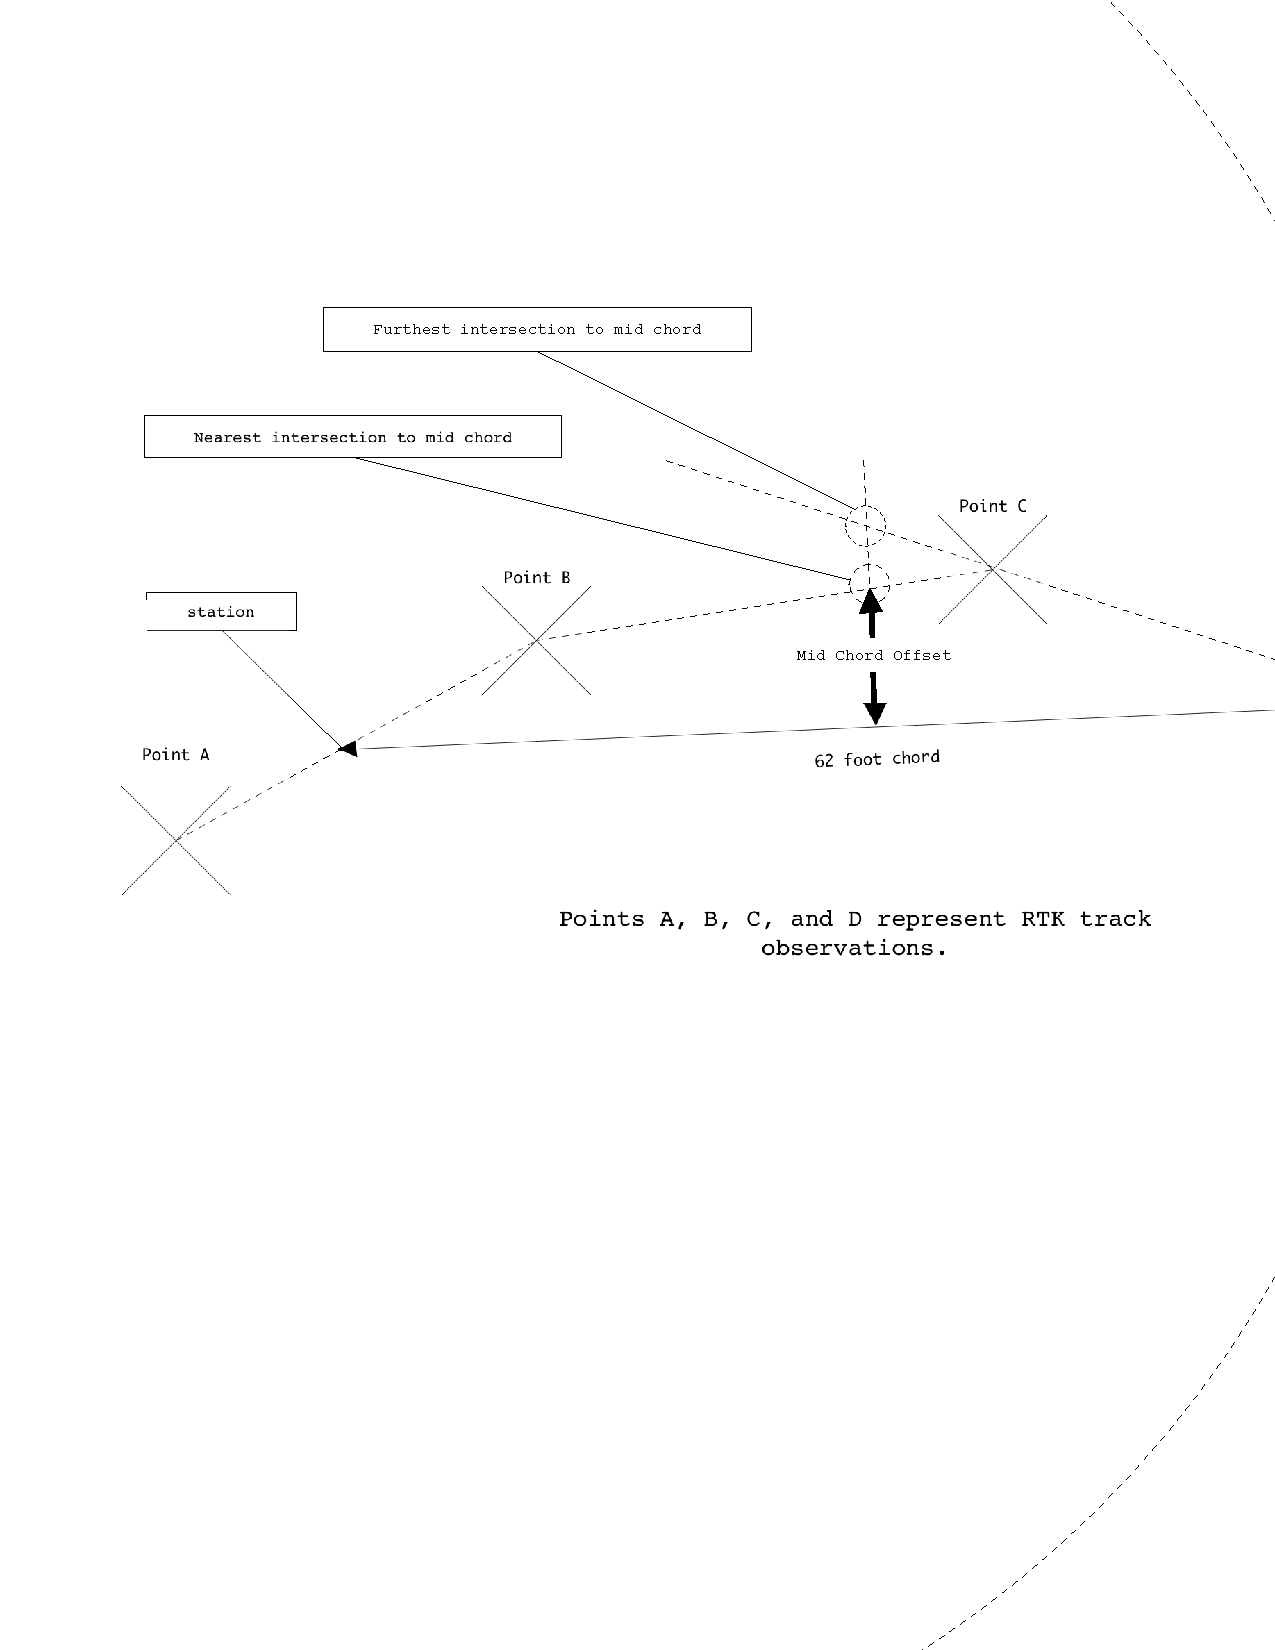
\includegraphics[width=13cm]{graphics/stringLining.png}
		\caption{Modeling the String Line Method from RTK Track Observations}
		\label{fig:strLine}
	\end{center}
\end{figure}

The MCO is determined from an line orthogonal with the mid point of the chord, and the mean of the intersection with the nearest and farthest of two lines projected from the three observations nearest to the middle ordinate (figure~\ref{fig:strLining} points B, C, and D). The distance from the chord mid point and the mean intersection determines the MCO. The degree of curve (chord definition) is then found from the MCO and chord length in feet by the relationship~\citep{1964hickerson}.
	\begin{equation}
		D_c = \frac{45840 \times MCO}{chord^2}
		\label{eqn:degOcrv}
	\end{equation}
	
The model assigns a mile post reference to $D_c$ using the location of the mean intersection and equation \ref{eq:accumSlopeD}.

The coordinates of the next station are found by intersecting the stationing distance in a similar fashion to the chord circle intersection. Figure~\ref{fig:strLining} illustrates determination of a 15.5 foot station. 

A railway can be described as a smooth, continuous shape. As an aid to exploring the $D_c$, a smoothing algorithm is applied to the $D_c$ verses mile post reference.  The \emph{rlowess}\footnote{The \emph{rlowess} method is a local regression using weighted linear least squares and a 1st degree polynomial model that assigns lower weight to outliers in the regression. The method assigns zero weight to data outside six mean absolute deviations~\citep{matlab09}.} method of the \emph{smooth} function in the Matlab \emph{Curve Fitting Toolbox}$^{TM}$ was selected as a data exploration tool.

RTK derived track alinements from multiple traverses were plotted and evaluated by:
\begin{itemize*}
	\item Determining descriptive statistics of a traverse over tangent track for both a specialized geometry car $D_c$ and a RTK equipmed Hi-Rail $D_c$. vs. mile post reference across identical tangent segments.
	\item Graphic correlation of $D_c$ across identical track segments for multiple traverses.
	\item Variability between degree of curve in selected tangent track segments modeled with RTK GNSS data against rail company provided track geometry vehicle data.
\end{itemize*}

Tangent segments were selected from the MP 209-207 GMRS data. The degree of curve variance was determined from the selected tangent segments.

% Track Occupancy Design
\subsection{Experiment Three: Determining Track Occupancy} 
This experiment asked whether a common track vehicle using RTK augmented GPS/GNSS was able determine track occupancy by obtaining position accuracy defined by the FRA for a location determination system. The FRA LDS requirement stated in \emph{Differential GPS: An Aid To Positive Train Control}~\citep{1995FRADiffe} page 6, establishes the criteria to\\
\begin{quotation}
``...determine which of two tracks a given train is occupying with a very high degree of assurance (an assurance that must be greater than 0.99999 or (0.9$_5$)). The minimum center-to-center spacing of parallel tracks is 11.5 feet...''\\
\end{quotation}
The FRA specification is interpreted here to mean an observation must have a cross-track error no greater than $\pm \frac{11.5}{2}$ feet within a confidence interval (1-${\alpha}$), where ${\alpha}$ = 0.00001 or 0.99999.

Several traverses of a parallel multitrack segment were made by RTK GNSS equipped Hi-Rail. A track segment was selected based on the length of the tangent or curve and existence of adjacent parallel track traverses. The first traverse was designated as a reference centerline, and the centerline coefficients for tangent track determined by regression using the Matlab function \emph{regress}.

In the tangent case, the Matlab function call took the general form: \emph{[b,bint,r,rint,stats] = regress (Northing, Easting, 1), ${\alpha}$}. 
The function output \emph{b} contained the coefficient estimates, \emph{bint} contains the upper and lower confidence bounds of the coefficient estimates, and \emph{r and rint} contain residuals and residual intervals that have no meaning in this analysis. The statistics contained in \emph{stats} contains ${R^2}$ statistic, the ${F}$ statistic and its p-value, and an estimate of the error variance.

The slope is converted to an azimuth and back bearing by the function \emph{slope2Az}, listed in Appendix B, page \pageref{software}. The azimuth of the tangent was verified using the graphical solution in the \emph{TGO} software.

The cross-track\footnote{Figure \ref{fig:trackRef} page \pageref{fig:trackRef}} distance between subsequent observations and the baseline was determined by the Matlab function \emph{perpDist2line}, listed in Appendix B, page \pageref{software}. The function determines the cross-track distance for all subsequent observations in the tangent segment using equation \ref{tanXtrack}.
%d = abs[(aX + bY +c)/srt(a^2 + b^2)]
\begin{equation}
d = \left|\frac{ax + by + c}{\sqrt{a^2 + b^2}}\right| \\
\label{tanXtrack}
\end{equation}
where a, b, c are the coefficients of the reference tangent, \emph{x} is the observation Easting and \emph{y} is the observation Northing.

For the circular curve case, the coefficients of the reference curve origin and radius are determined from Northing and Easting observation of the selected curve segment. The cross-track distance is determined by the difference between the circular curve radius and coordinate distance from the origin.

Circular curve coefficients were determined by the Matlab function \emph{regress}. The specific form

%crvAX = [crvA.easting*.2 crvA.northing*.2 numel(crv2.northing)*.-1]
%crvAY = [crvA.easting.^2 crvA.northing.^2]

% Tangent hypothesis test
The null hypothesis statement is the reference track is occupied if the distance between an RTK GNSS observation and the reference centerline is less than or equal to $\frac{11.5}{2}$ feet at a confidence of 100(1-${\alpha}$)\%. The Matlab function \emph{ztest}  was used for the z-test of the null hypothesis. The function output indicates whether the null hypothesis is a random sample from a normal distribution with mean distance ${\le}$ 5.75 feet and standard deviation $\sigma$, against the alternative that the mean is not ${\le}$ 5.75 feet. The result of the test is  indicates a rejection of the null hypothesis at the 100(1 - 0.00001)\% significance level.

\begin{equation}
	h_{0}: \mu_d \le \frac{11.5}{2}\\
\end{equation}
\begin{equation}
	h_{1}: \mu_d > \frac{11.5}{2}\\
\end{equation}

The null hypothesis asserts that the cross-track error population parameter is equal to or less than half the FRA centerline to centerline track spacing. Acceptance of the null hypothesis indicates statistical evidence exists to assert same track occupancy to the confidence interval specified by the FRA~\citep[pp. 6]{1995FRADiffe}.

Matlab command for regression statistics
input: y value, [x value, array of ones: numEl], alpha 
[b,bint,r,rint,stats] = regress(B.Northing,[B.Easting ones(numel(B.Easting),1)],0.00001)

The Matlab \emph{Statistics Toolbox} funtion \emph{ztest} performs a z-test of the null hypothesis that the cross-track error data is a random sample from a normal distribution with mean \emph{m} and standard deviation $\sigma$, against the alternative that the mean is not \emph{m}. The result of the test indicates a rejection of the null hypothesis at the (1-${\alpha}$) significance level.


Experiment three objectives sought to:
\begin{enumerate*}
	\item  Collect single epoch observations on a nominal 5 foot horizontal spacing with RTK augmented GPS on board a track vehicle over 29 continuous miles of mainline track.
	\item Determine the coefficients for the position of select tangent and circular track segments. Long tangent and circular segments will be selected to maximize the number of data.
	\item Determine the distance between subsequent observations by track vehicle to the reference tangent and curve segments.
	\item Determine if statistical evidence exists to indicate if RTK GNSS is capable of determining track occupancy of a vehicle meeting FRA performance standards for a location determination system.
\end{enumerate*}
% Variables
\emph{Variables of analysis}: The mobile instrument \#1 and \#2, table \ref{tab:inst} produced these variables:
\begin{itemize*}
	\item UTM, Zone 17 North, northing in US survey feet.
	\item UTM, Zone 17 North, easting in US survey feet.
	\item NAVD 88, height above ellipsoid, Geoid 2003, in US survey feet.
	\item Time (local, EST) and date of observation.
\end{itemize*}
% Instrumentation %
\section{Instrumentation}
Instruments used in the research are summarized in table \ref{tab:inst}.
% Table of instrumentation
\begin{center}
\begin{threeparttable}
	\caption{Instrumentation and Software}\label{tab:inst}
	\begin{tabular}{llll}%{ p{2.0cm} p{3cm} p{3cm} p{3cm}}
\toprule
	Designation & Instrument & Description &  Experiment\\
\midrule
	Ad hoc& Trimble 5700 & 24 ch. GPS receiver & 1\\
	Reference& Zephyr Geodetic & GPS antenna & \\
	Station& Trimmark III UHF radio & 450Mhz band, 25 watt& \\
\midrule
	CORS & NetRS/NetR5 & 24/72 ch. GPS\tnote{$\dagger$} /\-GNSS\tnote{$\ddagger$} & 2, 3\\
	& Trimble Zephyr Geodetic /2 & GPS/\-GNSS antenna &\\
	VRS & Trimble Network Infrastructure & Virtual Reference Station &\\
	& \emph{VRS} Net & version 2.83\tnote{$\dagger$} & 2, 3 \\
\midrule
	Static Module & Trimble R8 & 24 ch. GPS w/int. radio &1\\
	& Trimble TSC2 & Survey Controller &\\
\midrule
	Mobile\#1           & Trimble 5700 & 24 ch. GPS w/int. radio & 1\\
	& Trimble TSC2 & \emph{Survey Controller}v12.1x &\\
	& Trimble Zehyr & GPS antenna &\\
\midrule
	Mobile\#2                & Trimble R7 & 72 ch. GNSS receiver& 2, 3\\
	& Trimble TSC2       & \emph{Survey Controller}v12.1x &1, 2, 3\\
	& Trimble Zephyr 2 & GNSS antenna & 2, 3\\
\midrule
\multicolumn{3}{l}{Software}\\
	& National Geodetic Survey & Online User Positioning Service & 1 \\
	& Trimble \emph{Geomatic Office} & version 1.63 & 1, 2, 3 \\
	& Google Docs & Collaborative spreadsheet & 1\\
	& ESRI \emph{ArcMap}    & version 9.2     & 1 \\
	& Matlab 32-bit (maci)      &  version 7.8.0.347 (R2009a) & 1, 2, 3\\
	\bottomrule
	\end{tabular}
		\begin{tablenotes}
		\item[$\dagger$]{Owned and operated by the Ohio Department of Transportation, Aerial Mapping}
		\item[$\ddagger$]{Owned and operated by the N.J. Rahall Appalachian Transportation Institute}\\
		\end{tablenotes}
\end{threeparttable}
\end{center}

\begin{itemize*}
	\item An ad hoc reference station (AhRS) as listed in table \ref{tab:instruments} uses a stationary reference antenna to receive SV signals for manipulation by a GPS receiver to produce correctors for transmission over UHF data radio to a capable mobile GPS receiver.
	\item A single \emph{continuously operating reference station} (CORS) provides continuous data for RTK surveying applications.
	\item  A \emph{virtual reference station} (VRS) server provides differential positioning service across a large area from numerous CORS networked and synchronized with infrastructure software. Observations from each CORS in the network are pre-processed to generate models of the distance-dependent biases. Based on the model parameters and the user's approximate position, individual corrections can then be predicted, which enables differential positioning. The differential errors caused by ionospheric and tropospheric refraction, as well as satellite orbit errors are precisely estimated with networked RTK based on dual-frequency carrier phase observations regional network of CORS. Correction model parameters are determined to allow the prediction of the differential errors for the baseline between a master reference station and the user's position. Applying these corrections to code and carrier phase observations of the master reference station, VRS measurements are generated for RTK positioning of the rover receiver.
	\item A \emph{static survey} unit is an RTK enabled GPS or GNSS receiver used by a surveyor to determine the coordinate of a position by recording multiple-epoch observations while occupying the point of interest.
	\item A \emph{mobile survey unit} is an RTK enabled GPS orGNSS receiver used to determine the coordinates of a position while in motion by recording single epoch observations.
\end{itemize*}
			%%%%%%%%%%%%%%%%
			%  Data Validity and Integrity %
			%%%%%%%%%%%%%%%%
\section{Data Validity and Integrity}

% Validity
\emph{Validity}

Insuring the the validity of RTK GPS/GLONASS data relied on the quality control performed by the data collector software. A field notebook was kept to record various instrument and initial values (i.e., antenna height from top of rail, locomotive number, track points of interest) found during antenna alinement. The recorded values were programmed into the controller as a specific survey style to insure the use of identical calibration values between observation files during multi-day surveys and spanning months using a particular Hi-Rail.

The survey controller was programmed to reject observations that fell outside a threshold relative horizontal and vertical precision as determined by the receiver. A threshold value of 0.15 feet horizontal and 0.50 feet vertical was selected for the hump yard survey, and 0.10 feet horizontal and 0.20 feet vertical was selected for the alinement surveys. The threshold values were selected based on the manufacture's stated accuracy, the expected degradation due to reference station distance, the  receiver type, plus overhead. Receivers designated as GPS are capable of receiving and decoding only GPS SVs, while a GNSS receiver is capable of receiving GPS and GLONASS SVs. In all cases, the vertical threshold allowance is twice the horizontal value.

The hump yard observations were plotted using ESRI ArcMap software to produce color-mapped plan views of the yard. The color-mapped plot is similar to a contour map. However, where a contour map utilizes a triangulated irregular network to provide elevations over an area feature, the centerline top-of-rail line feature is of interest in a hump yard. Elevations were plotted as colored dots indicating an elevation range.

Color mapping relative vertical precision provides a graphical method of analysis for time-related SV reception quality. RTK GPS quality is dependent on satellite geometry, so serial observations of lower quality would be expected to appear together.

The track alinement model processes observations that are determined to be sequence by the software model. Changes in bearing between any two observations that approached 180$^{\circ}$ indicated the Hi-Rail reversed direction while recording of track observations. Points recorded in the reverse direction were not used.

% Integrity
\emph{Integrity}

During the hump yard experiment, several hundred points of interest\footnote{track switch points, retarder inlet and outlet, wheel detectors} (POI) were surveyed on the ground with the static survey instrument. The points were later translated such that the POI was relocated to the the track centerline.

Transferring the hump yard data to a CAD drawing used a web-based spreadsheet to enable  collaboration among the research team.

A check on point sequencing in the alinement model plots the sequence in three dimensions. The ordered sequence for each mile can be verified by examining the 3D plot.

% Summary
% Summary goes back to problem statement
\section{Summary}
The research method explores track measurement using commercial off-the-shelf RTK augmented GPS and GNSS instrumentation.  Each experiment examines the value of RTK augmentation to provide value in challenging railway measurements. The research examines the ability of single epoch RTK GNSS observations to act as a component of a location determination system.

Experiment 1 traversed an active hump yard with a locomotive equipped with RTK GPS instruments to observe track positions. The recorded positions were used to produce a profile for each track. The relative vertical precisions of the locomotive observations and reference station were analyzed for the influence of multipath reflections.

Experiment 2 traversed a continuous 29 mile segment of mainline track by a Hi-Rail equipped with RTK GNSS instruments. A model of the string line method was used to determine the ${D_c}$ for each mile, evaluate the model against rail company track charts for location, magnitude, and direction of curves. The model was used to 	evaluate the performance of RTK GNSS and the model against a specialized track geometry car over a comparable segment of tangent track.

Experiment 3 evaluated the ability to determine track occupancy by RTK GNSS. Five surveys traversed a parallel multitrack segment. The cross-track error between a baseline survey and subsequent surveys was evaluated in a tangent and circular curved segment. The statistical likelihood of estimating track occupancy meeting FRA guidelines for a location determination system was determined.

